\chapter{Layout Guidelines for an Activity Flow Maps}
\label{chp:af:layout}

\section{Introduction}

The previous chapters describe the appearance and meaning of \SBGNAFLone components. Objects are \glyph{activity nodes}, \glyph{container nodes}, \glyph{logical operators}, \glyph{submaps} as well as \glyph{connecting arcs}. The components of an \AFm have to be placed in a meaningful way -- a random distribution with spaghetti-like connections will most likely hide the information encoded in the underlying model, whereas an elegant placement of the objects, giving a congenial appearance of the maps, may reveal new insights. The arrangement of components in a map is called a \emph{layout}.

SBGN \AFs should be easily recognisable not only by the glyphs used, but also by the general style of the layout. However, the arrangement of the components is a complex art in itself, and there is no simple rule which can be applied to all cases. Therefore this
section provides rules, some of which are requirements and some are recommendations, for the layout of activity flow maps.
In addition, we provide a list of additional suggestions which may help in producing aesthetically more pleasant layouts, possibly easier to understand.

Those layout guidelines are independent of the method used to produce the map, and apply to both manually drawn maps as well as maps produced by an automatic layout algorithm. The guidelines do not deal with interactive aspects (\eg the effect of zooming). Further information about automatic network layout (graph drawing) can be found, for example, in the books of Di Battista and co-authors~\cite{DiBattista:1998} and Kaufmann and Wagner~\cite{Kaufmann:2001}.

Please note that the colour of objects do not carry any meaning in SBGN. Although one can use colours to emphasize part of a diagram or encode additional information, the meaning of the diagram should not depend on the colours. Furthermore, objects can have different sizes and size is also meaningless in SBGN. For example, one biological activity node may be larger than another node. Also the meaning of a graph should be conserved upon scaling as far as possible.

\newpage

\section{Layout guidelines}

\subsection{Requirements}

Requirements are rules which \textbf{must} be fulfilled by a layout to produce a valid \SBGNAFLone map.

\subsubsection{Node-node overlaps}
\label{af:NoNoOv}

Nodes are only allowed to overlap in two cases:
\begin{enumerate}
  \item the overlapping nodes define a glyph (\eg \glyph{auxiliary unit}).
  \item nodes overlapping compartments  (\eg a \emph{biological activity} placed on a compartment).
  \item compartment overlapping compartment (\eg,  \fig{overlap}). However, it should be noted that it does not have implication of containment of one compartment to the other.
\end{enumerate}
Otherwise, nodes are not allowed to overlap (\fig{af:layout1}). This includes the touching of nodes, which is also not allowed. Also submaps are not allowed to overlap.

\begin{figure}[!ht]
  \centering
  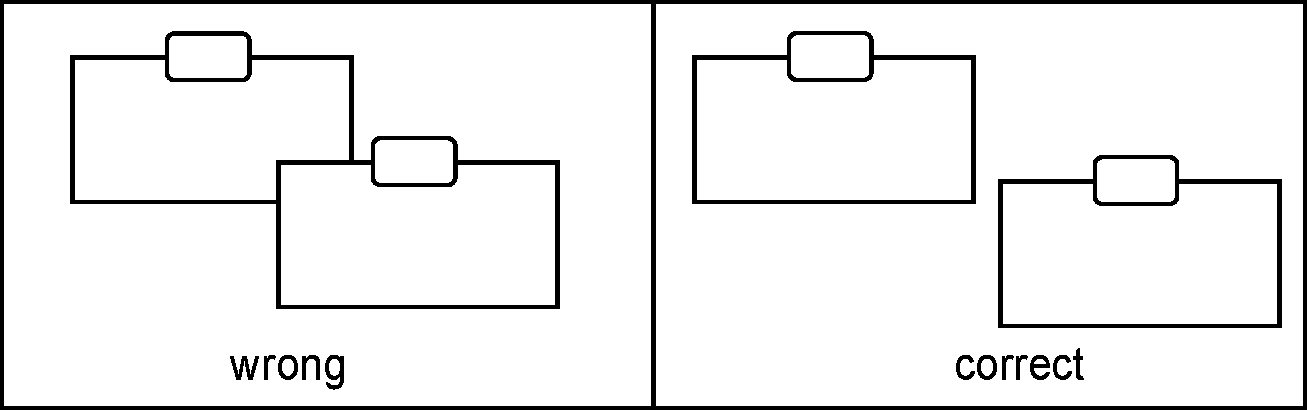
\includegraphics[scale=0.4]{images/build/layout-node-node.pdf}
  \caption{Nodes must not overlap.}\label{fig:af:layout1}
\end{figure}

\subsubsection{Node-edge crossing}
\label{af:crosEdNoRe}

In general, such crossing should be avoided.  In case this can't be avoided, the edge must be drawn on the top of the node (\fig{af:layout2}). See also recommendation \ref{af:crosEdNo} 

\begin{figure}[!ht]
  \centering
  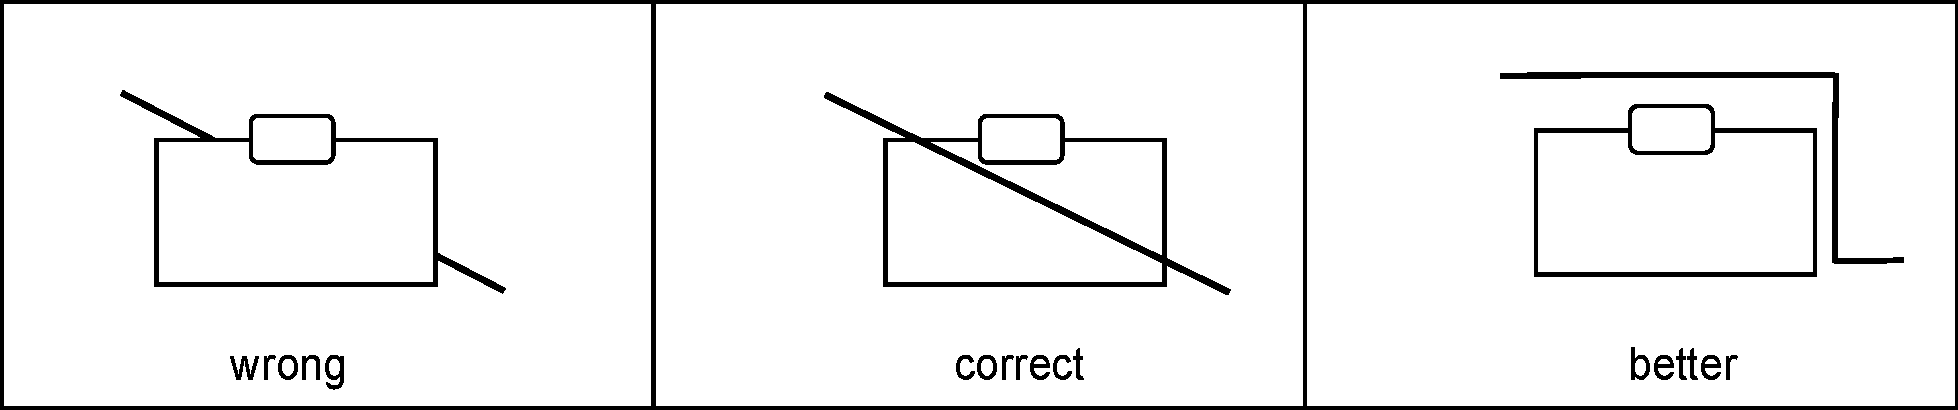
\includegraphics[scale=0.4]{images/build/layout-node-edge.pdf}
  \caption{If an edge crosses a node, the edge must be drawn on top  of the node.}\label{fig:af:layout2}
\end{figure}

\subsubsection{Node border-edge overlaps}

Edges are not allowed to overlap the border lines of nodes (\fig{af:layout3}).

\begin{figure}[!ht]
  \centering
  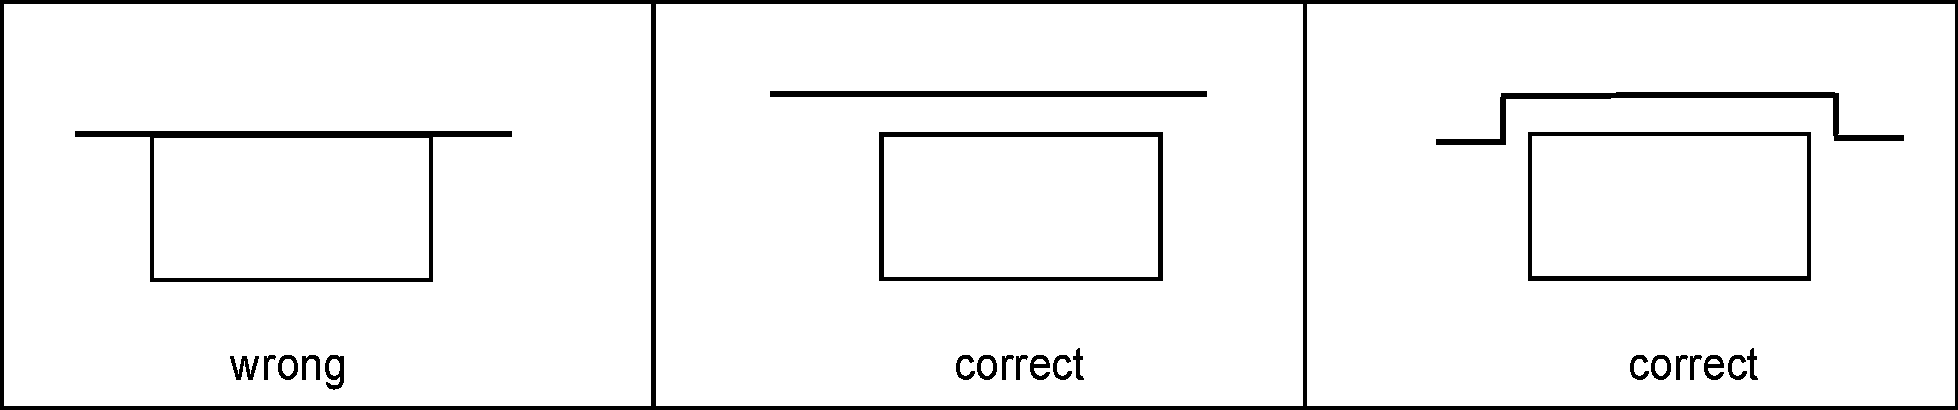
\includegraphics[scale=0.4]{images/build/layout-node-border-edge.pdf}
  \caption{Edges must not overlap node borders.}\label{fig:af:layout3}
\end{figure}

\subsubsection{Edge-edge overlaps}

Edges are not allowed to overlap (\fig{af:layout4}). This includes touching of edges. Furthermore, an edge is neither allowed to cross itself nor to cross
a boundary of node more than twice or other edges more than once.

\begin{figure}[!ht]
  \centering
  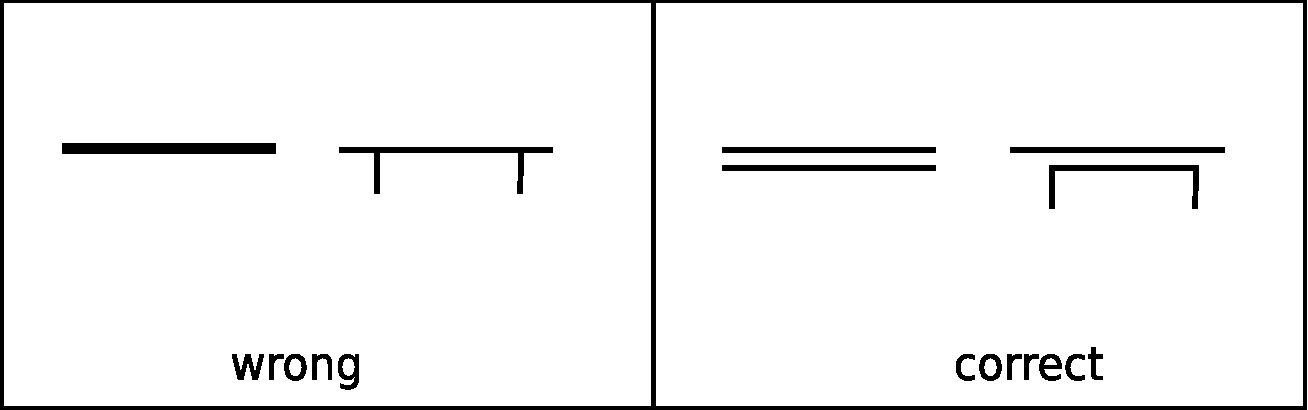
\includegraphics[scale=0.4]{images/layout-edge-edge}
  \caption{Edges must not overlap.}\label{fig:af:layout4}
\end{figure}

\subsubsection{Node orientation}

Nodes have to be drawn horizontally or vertically, any other rotation of elements is not allowed (\fig{af:layout5}).

\begin{figure}[!ht]
  \centering
  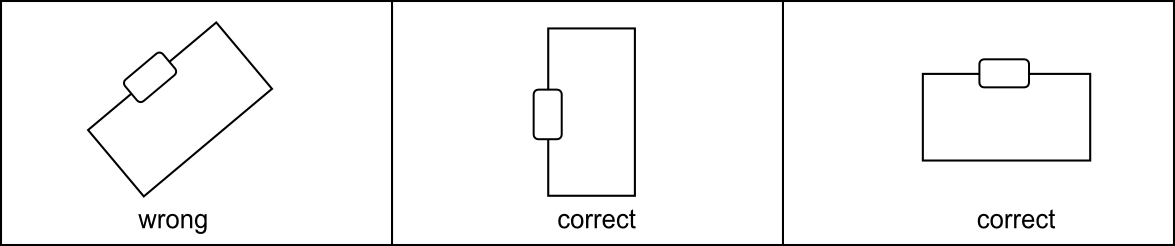
\includegraphics[scale=0.4]{images/layout-orientation}
  \caption{The node orientation must be horizontally or vertically.}\label{fig:af:layout5}
\end{figure}

\subsubsection{Node labels}

At least a part of the label (unbordered box containing a string of characters) has to be placed inside the node it belongs to. Node labels are not allowed to overlap nodes or other labels (this includes touching of other nodes or labels).

\subsubsection{Edge labels}

Edge labels are not allowed to overlap nodes. This includes touching of nodes.

\subsubsection{Compartments}

If a network has all participants (nodes and edges) in the same compartment, all the activity nodes and edges/arcs have to be in this compartment.  \\
Edges/arcs are allowed to cross the compartment boundaries when the input and output ANs are in two different compartments.

\subsection{Recommendations}

Recommendations are rules which should be followed if possible to produce layouts that are easier to understand.

\subsubsection{Node-edge crossing}
\label{af:crosEdNo}

Crossings between edges and nodes should be avoided. Some crossings may be unavoidable, \eg the crossing between an edge and a compartment border. See also requirement \ref{af:crosEdNoRe} (in case of node-edge crossings the edge must be drawn on the top of the node).

\subsubsection{Labels}

Labels should be horizontal. Node labels should be placed completely inside the node if possible. Edge labels should be placed close to the edge and avoid overlapping the edge as well as other edge labels.

\subsubsection{Avoid edge crossings}

The amount of crossings between edges should be minimized.

\subsection{Additional suggestions}

Here is a list of additional layout suggestions which may help in producing aesthetically more pleasing layouts which may be easier to understand.

\begin{itemize}
  \item Angle of edge crossings: If edge crossings are not avoidable   edges should cross with an angle close to 90 degrees.
  \item Drawing area and width/height ratio: The drawing should be compact and the ratio between the width and the height of the drawing should be close to 1.
  \item Edge length: Long edges should be avoided if possible.
  \item Number of edge bends: Edges should be drawn with as few bends as possible.
  \item Similar and symmetric parts: Similar parts of a map should be drawn in a similar way, and symmetric parts should be drawn symmetrically.
  \item Proximity information: Related elements (\eg nodes connected by edges within a compartment) should be drawn close together.
  \item Directional information: Subsequent activities (\eg a sequence of activities) should be drawn in one direction (\eg from top to bottom or from left to right).
  \item Compartments: Different compartments should have different background shade or colour.
\end{itemize}